\beginsong{Wir sind eine kleine verlorene Schar}[wuw={Alf Zschiesche, Nerother Wandervogel}, pfii={19}, bo={404}]

\beginverse
\endverse
\centering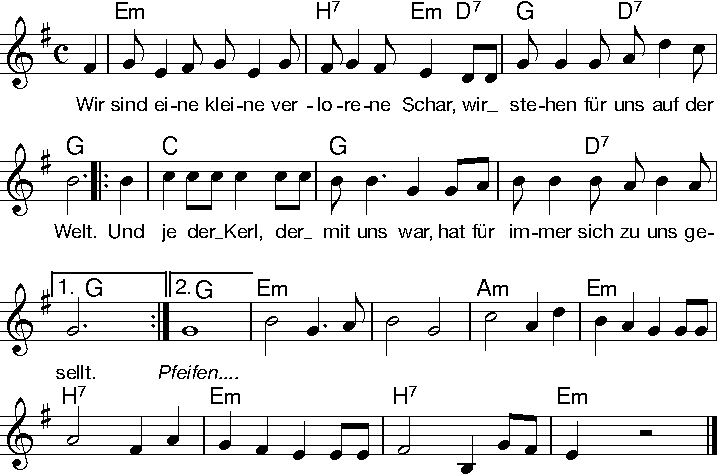
\includegraphics[width=1\textwidth]{Noten/Lied100.pdf}	

\beginverse
Wir \[Em]leben in Lumpen, wir \[H7]lieben die \[Em]Nacht, \[D7]uns're \[G]Zeit heißt \[D7]immer das \[G]Jetzt,
wir \[C]haben die Spießer \[G]ängstlich gemacht und wir lachen, \[D7]wenn man uns \[G]hetzt.
\endverse

\beginverse
So ^ziehen wir weiter durchs ^Land, durch die ^Zeit, ^wir ^ändern uns ^nimmer^mehr.
Lasst ^uns die Fahne, die ^Fahrt und das Scheit und den abge^brochenen ^Speer.
\endverse

\endsong

\beginscripture{} 
Lied über das Verbot der bündischen Jugend. ''...den abgebrochenen Speer'': Zum Selbstschutz wurden die Wimpespeere teilweise zerbrochen, so konnte man der Hitlerjugend entfliehen.
\endscripture
